\section{Introduction}
\label{sec:introduction}

Wavetable oscillators store a single period of a waveform and advance a read pointer modulo the table length.
When $x[0]\neq x[L-1]$, the wrap is a hard discontinuity that, under cyclic playback, becomes a periodic click with a broadband spectrum locked to the fundamental.
The same geometry appears whenever a short loop buffer is tiled for listening or for objective evaluation.
We define the repair task as \emph{cycle-local seam restoration}: edit a neighborhood of the wrap (and optionally a lightweight residual cell over the period) so that multi-period playback matches an ideal reference that never opens the wrap cliff.
That outer agreement is scored by the prolonged residual $R$ for this periodic seam artifact class.

Figure~\ref{fig:intro-sine} shows one real sine-wrap edge case from the frozen canonical holdout (same \texttt{make\_batch} tile, seed~\texttt{20260719}).
Four roles must stay distinct: (a)~ideal sibling $r^{\star}$ (cliff withheld; unscored target);
(b)~no-bake / cracked engine $x$ after open-wrap cliff ($R\approx 0.950$ vs $r^{\star}$; ideal overlay);
(c)~DualCosine classical bake on that same tile ($R\approx 0.603$ on this severe cliff);
(d)~Ours / DenoiseOpt favorite bake (\texttt{champion\_iter\_000235}, tile $R\approx 0.9917$).
Panels~(e)--(f) plot the modulation residual and a seam zoom so Ours is readable against DualCosine.
No-bake is not the ideal; DualCosine is one classical row (and separately a PPO advantage baseline; Section~\ref{sec:methods}).

\begin{figure*}[t]
  \centering
  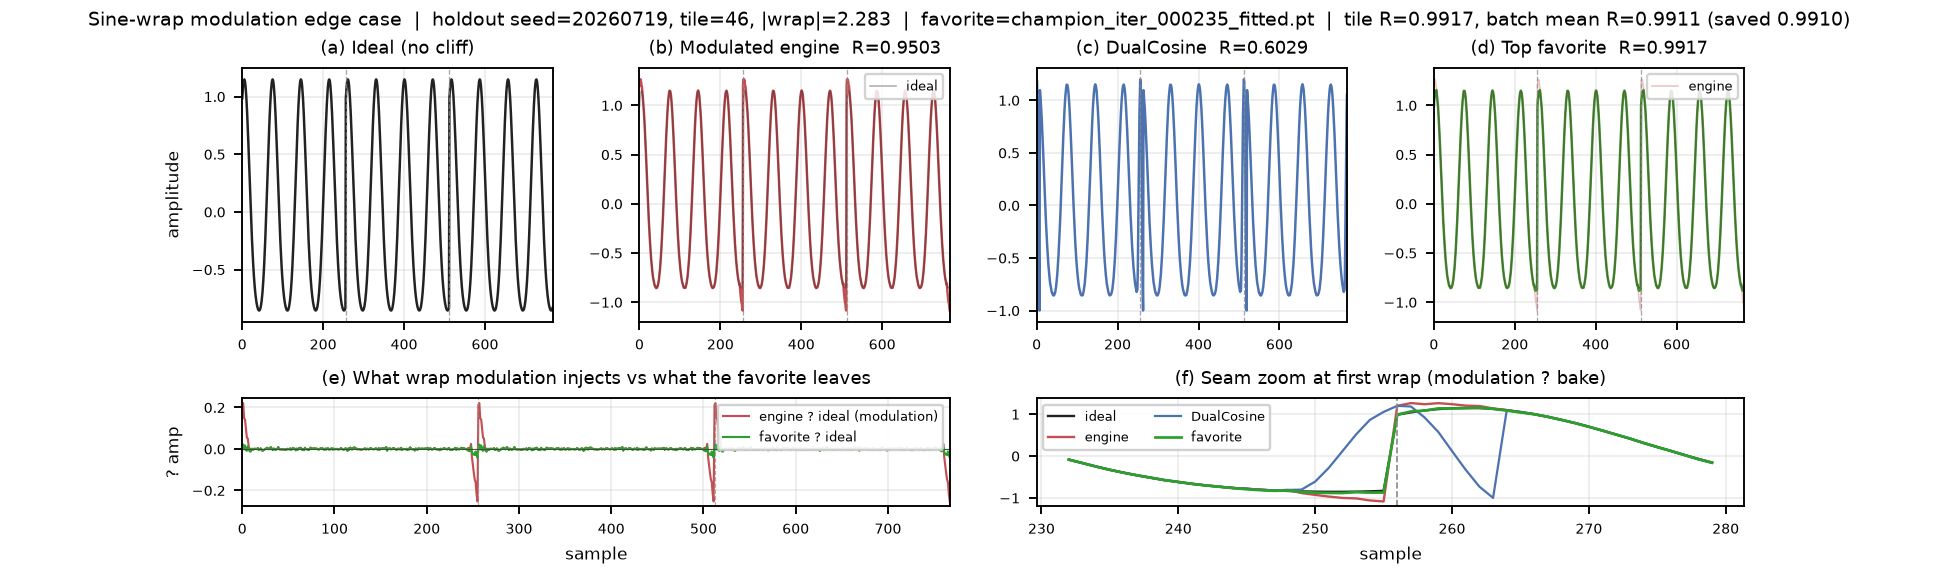
\includegraphics[width=\textwidth]{figures/fig_intro_sine_problem.png}
  \caption{Canonical holdout sine-wrap edge case (seed~\texttt{20260719}, $L{=}256$, $N{=}16$ tiles, same tile across panels).
  Distinguish four roles: (a)~ideal sibling $r^{\star}$ (cliff withheld; scoring target, not a method);
  (b)~no-bake / cracked engine $x$ (passthrough $\Theta{=}{\mathrm{id}}$, scored vs~$r^{\star}$);
  (c)~DualCosine classical end-fade bake;
  (d)~Ours (DenoiseOpt favorite bake).
  (e)--(f)~Modulation residual and seam zoom.
  Prolonged residual $R\in[0,1]$ (1~=~best) is printed per panel where scored.
  Accessibility: six-panel waveform comparison of ideal, no-bake, DualCosine, and Ours.}
  \label{fig:intro-sine}
\end{figure*}

Classical virtual-analog practice already supplies seam-local tools.
Alias-free BLIT/BLEP-style synthesis~\cite{stilson1996}, PolyBLEP / fractional-delay antialiasing~\cite{nam2009polyblep}, and BLAMP corner corrections~\cite{esqueda2016blamp} reduce wrap and geometric discontinuity energy in-band.
Those operators act locally; we score cycle-local bake approximations of them beside DualCosine (Section~\ref{sec:va-seam-baselines}).
They leave open which bake parameters and which residual cell, if any, minimize prolonged tiled error against a no-cliff ideal.
Label-free restoration work such as Noise2Noise shows that useful reconstructors can be ranked without paired clean targets when the evaluation geometry is explicit~\cite{lehtinen2018}.
Speech-domain Noise2Noise denoisers extend that idea to audio waveforms~\cite{kashyap2021n2n}.
Mixture-invariant unsupervised separation likewise avoids paired clean stems for ranking~\cite{wisdom2020}.
On the search side, NAS surveys~\cite{elsken2019}, RL controllers~\cite{zoph2017nas,pham2018}, aging evolution~\cite{real2017large,real2019}, population-based hyperparameter schedules~\cite{jaderberg2017}, CMA-ES tutorials~\cite{hansen2016cmaes}, and evolution-guided policy gradients~\cite{khadka2018} motivate a hybrid outer loop: GA for population diversity, PPO for discrete architecture edits~\cite{schulman2017}, and PBT-style exploit--mutate on elites.
Platform-aware and progressive NAS add compute-aware search priors~\cite{tan2019mnasnet,liu2018pnas}.
MoE soft gates suggest routing among heterogeneous tiny cells under one residual score~\cite{shazeer2017}.
Waveform separation nets (Wave-U-Net, Conv-TasNet, dual-path RNN, SepFormer) and audio DL surveys inform the searchable cell family at bake-scale width~\cite{stoller2018,macartney2018,luo2019,luo2020dprnn,subakan2021,purwins2019,gong2021ast}, with U-Net / ResNet / attention primitives as block ancestors~\cite{ronneberger2015,he2016resnet,vaswani2017,jansson2017}.

The contribution is a meta-learning protocol for this periodic seam instance.
An outer RL+GA(+PBT) loop proposes bake-cell operator graphs and continuous bake parameters.
Each candidate is scored by prolonged residual $R\in[0,1]$ (1~=~best) between engine-baked multi-period audio and a procedural ideal sibling $r^{\star}=G(\mathrm{seed},\mathrm{cliff{=}off})$.
Paired studio-clean wavetables are not required for every trial.
Differentiable DSP modules~\cite{engel2020} place DualCosine / FIR / MLP seam ops in an interpretable stack.
Bayesian HPO~\cite{snoek2012} informs prior families that compete under the same $R$.
A CUDA hybrid search campaign (PPO+GA+PBT+NAS, depth and MoE biases) has passed a $5{,}000$-iteration clean gate with champion $R\approx 0.9909$ versus DualCosine $\approx 0.8166$ on the runner geometry.
The frozen canonical holdout and inference benches in Section~\ref{sec:results} are the measured evaluation matrices for this report.
Primary claim scope is cycle-local wavetable seam restoration (DAFx / AES / arXiv cs.SD).
We do not claim speech enhancement, music source-separation, or deep SOTA on classical sci/eng transfer boards.

\subsection{Contributions}
\label{sec:contributions}
\begin{enumerate}
  \item \textbf{Problem framing.} Cast wavetable wrap discontinuity as cycle-local seam restoration under prolonged tiled evaluation, separating seam-local diagnostics from residual $R$.
  \item \textbf{Hybrid DenoiseOpt outer loop.} Specify RL+GA(+PBT) search over discrete operator graphs and continuous bake parameters, with named branches (GA crossover, PPO mutation, PBT exploit, MoE soft gates).
  \item \textbf{Formal residual protocol.} Define bake operator $\Theta$, ideal-sibling generator $G$, outer objective $\max R(y,r^{\star})$, and reimplementable Algorithms~\ref{alg:residual}--\ref{alg:hybrid} (Appendix~\ref{app:algorithms}). No wrap-closure or search-convergence guarantees.
  \item \textbf{Open evaluation path.} Release companion code for the synthesizer engine and meta search, with frozen $5$k-gate figures, hard-cliff strata, N2N/seq baselines, and wavetable-native transfer benches.
\end{enumerate}

Section~\ref{sec:related_work} organizes related work by mechanism.
Sections~\ref{sec:methods}--\ref{sec:experiments} detail the residual objective and search protocol.
Section~\ref{sec:results} reports the $5$k-gate freeze and inference benches.
